\documentclass[10.5pt,compress]{beamer}
\usepackage[utf8]{inputenc}
\usepackage[T1]{fontenc}
\usepackage{lmodern}
\usepackage{tikz}
\usetikzlibrary{patterns}
\usepackage{tikz-cd}
%\tikzset{commutative diagrams/arrow style=math font}

% Beamer commands
\title{The Yoneda Lemma}
%\setbeamertemplate{navigation symbols}{}
%\setbeamertemplate{blocks}[rounded][shadow=false]
%\usecolortheme{orchid}
% TikZ options
\usetikzlibrary{arrows,shapes}
\useoutertheme{split}
\useoutertheme[footline=authortitle]{miniframes}
%\useinnertheme{circles}
%\usecolortheme{whale}
%\usecolortheme{orchid}

\definecolor{beamer@blendedblue}{rgb}{0.3,0.5,0.8}
\definecolor{beamer@myviolet}{rgb}{0.7,0.2,0.5}
\definecolor{beamer@deepblue}{rgb}{0.5,0.5,0.7}
\definecolor{beamer@lightgray}{rgb}{0.5,0.7,0.5}
\definecolor{beamer@mybrown}{rgb}{0.3,0.3,0.2}
\definecolor{beamer@mathtext}{rgb}{0.9,0.5,0.4}
\definecolor{beamer@header}{rgb}{0.4,0.1,0.1}

\setbeamercolor{background canvas}{fg=white, bg=black}
\setbeamercolor{normal text}{fg=beamer@lightgray,bg=black}
\setbeamercolor{alerted text}{fg=red}
\setbeamercolor{example text}{fg=green!50!black}
\setbeamercolor{miniframes}{fg=red,bg=white}
\setbeamercolor{structure}{fg=beamer@deepblue}
\setbeamercolor{titlelike}{fg=magenta}
\setbeamercolor{frametitle}{fg=beamer@myviolet}
\setbeamercolor{title}{fg=beamer@myviolet}
\setbeamercolor{item}{fg=beamer@mybrown}
\setbeamercolor{section in head/foot}{fg=white,bg=beamer@header}

\setbeamerfont{framesubtitle}{size=10pt}


\mode
<all>

%\setbeamercovered{invisible}
\begin{document}

\begin{frame}\label{frame : titlepage}
\titlepage
\end{frame}

%%%%%%%%%%%%%%%%%%%%%%%%%%%%%%%%%%%%%%%%%%%%%%%%%%%%%%%%%%%%%%%%%%%%%%%%%%%%%%%%%%%%%%%%%%
\section{Representable Functors}
\begin{frame}\label{frame : representable functors}
\frametitle{Representable Functors}

\begin{definition}[Representation of a functor]
\begin{enumerate}

\item[$\blacktriangleright$]
A representation of a covariant functor $F : C \to Set$ consists of an object $c \in C$ 
along with a natural isomorphism $\alpha : Hom(c,-) \cong F$.\smallskip

\item[$\blacktriangleright$] 
Dually, A representation of a contravariant functor $F : C \to Set$ consists of an object 
$c \in C$ along with a natural isomorphism $\alpha : Hom(-,c) \cong F$.\smallskip

\item[$\blacktriangleright$]
A funtor is representable if it has a representation.

\item[$\blacktriangleright$]
For issues with size, we need $C$ to be locally small.

\end{enumerate}

\end{definition}
\end{frame}

%%%%%%%%%%%%%%%%%%%%%%%%%%%%%%%%%%%%%%%%%%%%%%%%%%%%%%%%%%%%%%%%%%%%%%%%%%%%%%%%%%%%%%%%%%%%%%
\begin{frame}\label{frame : eg of cov rep func}
\frametitle{Examples}

\begin{block}{Covariant representable functors}
\begin{enumerate}

\item[$\blacktriangleright$] The identity functor $id : Set \to Set$ is represented by
the singleton set $\mathbf{1}$. That is, for a set $X$
$Hom(\mathbf{1}, X) \cong X$.

\item[$\blacktriangleright$] The forgetful functor $U : Group \to Set$ is represented by
$\mathbb{Z}$.

\item[$\blacktriangleright$] The forgetful functor $U : Top \to Set$ is represented by the
singleton space.

\item[$\blacktriangleright$] The functor $Path : Top \to Set$ which maps a topological space
$X$ to its set of paths is represented by the unit interval $I$.
\end{enumerate}

\end{block}

\end{frame}

%%%%%%%%%%%%%%%%%%%%%%%%%%%%%%%%%%%%%%%%%%%%%%%%%%%%%%%%%%%%%%%%%%%%%%%%%%%%%%%%%%%%%%%%%%%%%%%

\begin{frame}[fragile]\label{frame : eg of contra rep func}

\frametitle{Examples}

\begin{block}{Contravariant representable functors}
\begin{enumerate}

\item[$\blacktriangleright$] 
The contravariant power set functor $P : Set^{op} \to Set$ is represented by the set
$\mathbf{2} = \{\top, \bot\}$. That is $Hom(X,\mathbf{2}) \cong P(X)$.

\item[$\blacktriangleright$] 
The functor $\mathcal{O} : Top^{op} \to Set$ which maps a topological space to its
set of open subsets is represented by the Sierpienski space $S$.
\begin{equation*}
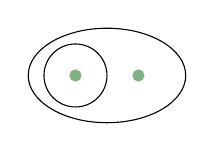
\begin{tikzpicture}
\draw (2,2) ellipse (1cm and 0.6cm);
\draw (1.6,2) circle (0.4cm);
\draw[beamer@lightgray,fill = beamer@lightgray] (1.6,2) circle (0.07cm);
\draw[beamer@lightgray,fill = beamer@lightgray] (2.4,2) circle (0.07cm);
\end{tikzpicture}
\end{equation*}

\item[$\blacktriangleright$]
The functor $D : Vect_K^{op} \to Set$ which maps a vector space to its dual is represented by
$K$, considered as a vector space on itself.

\end{enumerate}

\end{block}

\end{frame}

%%%%%%%%%%%%%%%%%%%%%%%%%%%%%%%%%%%%%%%%%%%%%%%%%%%%%%%%%%%%%%%%%%%%%%%%%%%%%%%%%%%%%%%%%%%%%%%

\section{The Yoneda Lemma}
\begin{frame}\label{frame : yoneda lemma}

\begin{theorem}[The Yoneda lemma]
\only<1>{
For a locally small category $C$ and a covariant functor $F : C \to Set$, 
there is a bijection
\textcolor{beamer@mathtext}{
\[ \Phi_c^F : Nat(Hom(c,-), F) \cong Fc .\]
}
It maps a natural transformation $\alpha : Hom(c,-) \implies F$ to the element 
$\alpha_c(id_c)$, and is natural in both $c$ and $F$.\smallskip
}
\only<2>{
Dually, for a locally small category $C$ and a contravariant functor $F : C \to Set$, 
there is a bijection
\textcolor{beamer@mathtext}{
\[ \Phi_c^F : Nat(Hom(-,c), F) \cong Fc .\]
}
It maps a natural transformation $\alpha : Hom(-,c) \implies F$ to the element 
$\alpha_c(id_c)$, and is natural in both $c$ and $F$.\smallskip
}
\end{theorem}


\end{frame}
%%%%%%%%%%%%%%%%%%%%%%%%%%%%%%%%%%%%%%%%%%%%%%%%%%%%%%%%%%%%%%%%%%%%%%%%%%%%%%%%%%%%%%%%%%%%%%%

\begin{frame}[fragile]\label{frame : proof of covariant yoneda}
\begin{proof}[Proof(Covariant case)]
\color{beamer@mathtext}{
\begin{equation*}
\begin{tikzcd}
Hom(c,c) \arrow[r,"f*"] \arrow[d, "\alpha_c"] & Hom(c,d) \arrow[d, "\alpha_d"'] \\
Fc \arrow[r,"Ff"] & Fd"
\end{tikzcd} 
\begin{tikzcd}
id_c \arrow[r,"f*",mapsto] \arrow[d, "\alpha_c",mapsto] & 
f \arrow[d, "\alpha_d"', mapsto] \\
\alpha_c(id_c) \arrow[r,"Ff",mapsto] & \alpha_d(f)
\end{tikzcd}
\end{equation*}
}
\end{proof}
\end{frame}

%%%%%%%%%%%%%%%%%%%%%%%%%%%%%%%%%%%%%%%%%%%%%%%%%%%%%%%%%%%%%%%%%%%%%%%%%%%%%%%%%%%%%%%%%%%%%%%

\begin{frame}[fragile]\label{frame : naturality in the functor}
\begin{proof}[Naturality in the functor]
\[\beta : F \implies G \]
\[\beta_*(\alpha) = \beta \circ \alpha \]
\color{beamer@mathtext}{
\begin{equation*}
\begin{tikzcd}
Nat(Hom(c,-),F) \arrow[r,"\Phi^F"] \arrow[d, "\beta_*"] & Fc \arrow[d, "\beta_c"'] \\
Nat(Hom(c,-),G) \arrow[r,"\Phi^G"] & Gc"
\end{tikzcd} 
\begin{tikzcd}
\alpha \arrow[r,"\Phi^F",mapsto] \arrow[d, "\beta_*",mapsto] & 
\alpha_c(id_c) \arrow[d, "\beta_c"', mapsto] \\
\beta \circ \alpha \arrow[r,"\Phi^G",mapsto] & \beta_c \circ \alpha_c (id_c)
\end{tikzcd}
\end{equation*}
}
\end{proof}
\end{frame}

%%%%%%%%%%%%%%%%%%%%%%%%%%%%%%%%%%%%%%%%%%%%%%%%%%%%%%%%%%%%%%%%%%%%%%%%%%%%%%%%%%%%%%%%%%%%%%%
\begin{frame}[fragile]\label{frame : naturality in the object}
\begin{proof}[Naturality in the object]
\[f : c \to d \]
\[f^* : Hom(d,-) \implies Hom(c,-) \]
\[(f^*)^* : Nat(Hom(c,-),F) \longrightarrow Nat(Hom(d,-),F) \]
\color{beamer@mathtext}{
\begin{equation*}
\begin{tikzcd}
Nat(Hom(c,-),F) \arrow[r,"\Phi_c"] \arrow[d, "(f^*)^*"] & Fc \arrow[d, "Ff"'] \\
Nat(Hom(d,-),F) \arrow[r,"\Phi_d"] & Fd
\end{tikzcd}
\end{equation*}}
\end{proof}
\end{frame}

%%%%%%%%%%%%%%%%%%%%%%%%%%%%%%%%%%%%%%%%%%%%%%%%%%%%%%%%%%%%%%%%%%%%%%%%%%%%%%%%%%%%%%%%%%%%%%%

\begin{frame}[fragile]\label{frame : naturality in the object cont.}
\begin{proof}[Naturality in the object]
\color{beamer@mathtext}{
\begin{equation*} 
\begin{tikzcd}
\alpha \arrow[r,"\Phi_c",mapsto] \arrow[d, "(f^*)^*",mapsto] & 
\alpha_c(id_c) \arrow[d, "Ff"', mapsto] \\
(f^*)^*(\alpha) \arrow[r,"\Phi_d",mapsto] & 
((f^*)^*(\alpha))_d(id_d)) = Ff(\alpha_c(id_c))
\end{tikzcd}
\end{equation*}}
\color{beamer@lightgray}{
$((f^*)^*(\alpha))_d(id_d)) =
 (\alpha_d \circ f^*)(id_d) = 
  \alpha_d(f) = Ff(\alpha_c(id_c))$}
\end{proof}
\end{frame}

%%%%%%%%%%%%%%%%%%%%%%%%%%%%%%%%%%%%%%%%%%%%%%%%%%%%%%%%%%%%%%%%%%%%%%%%%%%%%%%%%%%%%%%%%%%%%%%

\begin{frame}[fragile]\label{frame : Natural transformations of hom-functors}
\frametitle{Natural transformations of $Hom$-functors}

For $f : c \to d$
Define $f_* : Hom(-,c) \implies Hom(-,d)$ as
\[ (f_*)_b = g \mapsto (f \circ g) : Hom(b,c) \to Hom(b,d) \]
Then if $h : a \to b$, the following commutative diagram says $f_*$ 
is a natural transformation
\color{beamer@mathtext}{
\begin{equation*}
\begin{tikzcd}
Hom(b,c) \arrow[r,"- \circ h"] \arrow[d, "(f_*)_b"] & 
Hom(a,c) \arrow[d, "(f_*)_a"'] \\
Hom(b,d) \arrow[r,"- \circ h"] & Hom(a,d)
\end{tikzcd}\hspace{20pt}
\begin{tikzcd}
g \arrow[r] \arrow[d] & g \circ h \arrow[d] \\
f \circ g \arrow[r] & f \circ g \circ h
\end{tikzcd}
\end{equation*}}
\color{beamer@lightgray}{
One can similarly define $f^* : Hom(d,-) \implies Hom(c,-)$.
}
\end{frame}

%%%%%%%%%%%%%%%%%%%%%%%%%%%%%%%%%%%%%%%%%%%%%%%%%%%%%%%%%%%%%%%%%%%%%%%%%%%%%%%%%%%%%%%%%%%%%%%

\section{The Yoneda Embedding}
\begin{frame}[fragile]\label{frame : the yoneda embedding}

\frametitle{The Yoneda Embedding}

The following define full and faithful embeddings:

\color{beamer@mathtext}{
\begin{equation*}
\begin{tikzcd}
	C \arrow[r, "Y", hook] & Set^{C^{op}}\\
    c \arrow[r, mapsto] \arrow[d, "f" '] & Hom(-,c) \arrow[d, "f_*"] \\
    d \arrow[r, mapsto] & Hom(-,d)	 
\end{tikzcd} \hspace{20pt}
\begin{tikzcd}
	C^{op} \arrow[r, "Y", hook] & Set^{C}\\
    c \arrow[r, mapsto] \arrow[d, "f" '] & Hom(c,-)  \\
    d \arrow[r, mapsto] & Hom(d,-)	\arrow[u, "f_*" '] 
\end{tikzcd}
\end{equation*}}
\end{frame}

%%%%%%%%%%%%%%%%%%%%%%%%%%%%%%%%%%%%%%%%%%%%%%%%%%%%%%%%%%%%%%%%%%%%%%%%%%%%%%%%%%%%%%%%%%%%%

\begin{frame}\label{frame : proof of faithfulness}
\begin{proof}[Proof of faithfulness]
For $f, g : c \to d$, $f_* = g_*$ implies 
 \[f = (f_*)_c(id_c) = (g_*)_c(id_c) = g \]  

\end{proof}
\end{frame}

%%%%%%%%%%%%%%%%%%%%%%%%%%%%%%%%%%%%%%%%%%%%%%%%%%%%%%%%%%%%%%%%%%%%%%%%%%%%%%%%%%%%%%%%%%%%%

\begin{frame}[fragile]\label{frame : proof of fullness}
\begin{proof}[Proof of fullness]
Using the Yoneda lemma with $F = Hom(-,d)$ we get
\[ \Phi^{Hom(-,d)}_c : Hom(c,d) \cong Nat(Hom(-,c), Hom(-,d)). \]
\end{proof}
\end{frame}

%%%%%%%%%%%%%%%%%%%%%%%%%%%%%%%%%%%%%%%%%%%%%%%%%%%%%%%%%%%%%%%%%%%%%%%%%%%%%%%%%%%%%%%%%%%%%

\section{Consequences}\label{frame : uniqueness of representations}
\begin{frame}
\frametitle{Uniqueness of representations}

If $Hom(c,-) \cong F \cong Hom(d,-)$ then using Yoneda lemma there is an unique
isomorphism $f : c \to d$ giving this particular natural isomorphism.
\end{frame}

%%%%%%%%%%%%%%%%%%%%%%%%%%%%%%%%%%%%%%%%%%%%%%%%%%%%%%%%%%%%%%%%%%%%%%%%%%%%%%%%%%%%%%%%%%%%%%


\begin{frame}[fragile]\label{frame : alt proof of Cayley's theorem}

\frametitle{An alternate proof of Cayley's theorem}
\begin{block}{Any group is isomorphic to a subgroup of a permutation group}
\smallskip
Consider a group $G$ as a category $BG$ with a single object $*$, and morphisms $g \in G$ with 
multiplication as composition. Using the Yoneda embedding each $g \in G$ 
induces an automorphism of $Hom(*,*) = G$. But functoriality and faithfulness implies 
that $g \mapsto g*$ is a group monomorphism. So $G$ is a subgroup of the
permutation group of $Hom(*,*)$. 
\color{beamer@mathtext}{
\begin{equation*} 
\begin{tikzcd}
* \arrow[r,"g"] \arrow[d,dashed] & * \arrow[d, dashed] \\
Hom(*,*) \arrow[r,"g^*"] & Hom(*,*)
\end{tikzcd}
\end{equation*}}


\end{block}	
	
\end{frame}

%%%%%%%%%%%%%%%%%%%%%%%%%%%%%%%%%%%%%%%%%%%%%%%%%%%%%%%%%%%%%%%%%%%%%%%%%%%%%%%%%%%%%%%%%%%%%%

\begin{frame}\label{frame : properties of C hat}
\frametitle{Some nice properties of $\widehat{C} = Set^{C^{op}}$}

\only<1>{
$\widehat{C}$ has small limits and co-limits. For a small diagram $F : I \to \widehat{C}$ 
\textcolor{beamer@mathtext}{
\[ (\lim_{\to} F(i))(U) = (\lim_{\to}F(i)(U)) \]
}
Specifically $\widehat{C}$ has products and co-products indexed over a set.
And hence also pullbacks, pushouts and equalizers.
}

\only<2>{
$\widehat{C}$ has exponentials when $C$ is small. For $A, B : C^{op} \to Set$ we have
\textcolor{beamer@mathtext}{
\[ B^A(I) \cong Nat(Y(I), B^A) \cong Nat(Y(I) \times A, B) \]
}
The first isomorphism follows directly from the Yoneda lemma.
The second isomorphism follows if we assume that exponentials exists. 
Since it is well formed, this actually gives a definition of the exponential.
}


\end{frame}

%%%%%%%%%%%%%%%%%%%%%%%%%%%%%%%%%%%%%%%%%%%%%%%%%%%%%%%%%%%%%%%%%%%%%%%%%%%%%%%%%%%%%%%%%%%%%%

\begin{frame}
\frametitle{One special case}\label{frame : alt defn of reals}

Take $C = (\mathbb{Q}, \leq)$. Instead of $Set$ take $\mathbf{2} = \{\emptyset, \{\emptyset\}\}$.
Then $2^{C^{op}} \cong \mathbb{R}$.

\end{frame}

%%%%%%%%%%%%%%%%%%%%%%%%%%%%%%%%%%%%%%%%%%%%%%%%%%%%%%%%%%%%%%%%%%%%%%%%%%%%%%%%%%%%%%%%%%%%%%

\begin{frame}[fragile]\label{frame : picking an element}
\frametitle{Set like constructions}

\begin{block}{Picking an element}
\color{beamer@mathtext}{
\begin{equation*} 
\begin{tikzcd}
1 \arrow[r,"a"] \arrow[rd,"f(a)" '] & A \arrow[d,"f"] \\
 & B
\end{tikzcd}
\end{equation*}}
\end{block}

\end{frame}


%%%%%%%%%%%%%%%%%%%%%%%%%%%%%%%%%%%%%%%%%%%%%%%%%%%%%%%%%%%%%%%%%%%%%%%%%%%%%%%%%%%%%%%%%%%%%%

\begin{frame}[fragile]\label{frame : union and intersection}
\frametitle{Set like constructions}

\begin{block}{Union is same as co-product. Intersection can be thought as the following
pullback diagram}
\color{beamer@mathtext}{
\begin{equation*} 
\begin{tikzcd}
A\cap B \arrow[r,dashrightarrow] \arrow[d,dashrightarrow] 
\arrow[dr, phantom,"\lrcorner", very near start]
& A \arrow[d,"i_A"] \\
B \arrow[r,"i_B"] & A\cup B
\end{tikzcd}
\end{equation*}}
\end{block}

\end{frame}


%%%%%%%%%%%%%%%%%%%%%%%%%%%%%%%%%%%%%%%%%%%%%%%%%%%%%%%%%%%%%%%%%%%%%%%%%%%%%%%%%%%%%%%%%%%%%%

\begin{frame}[fragile]\label{frame : subsets}
\frametitle{Set like constructions}

\begin{block}{Subsets can be thought as the following pullback diagram}
\color{beamer@mathtext}{
\begin{equation*} 
\begin{tikzcd}
A \arrow[r,dashrightarrow] \arrow[d,dashrightarrow] 
\arrow[dr, phantom,"\lrcorner", very near start]
& 1 \arrow[d] \\
X \arrow[r,"\mathcal{X}_A"] & 2
\end{tikzcd}
\end{equation*}}
\end{block}

\end{frame}


%%%%%%%%%%%%%%%%%%%%%%%%%%%%%%%%%%%%%%%%%%%%%%%%%%%%%%%%%%%%%%%%%%%%%%%%%%%%%%%%%%%%%%%%%%%%%%

\begin{frame}[fragile]\label{frame : pullback}

\frametitle{Pullback}

\color{beamer@mathtext}{
\begin{equation*}
\begin{tikzcd}
R
\arrow[drr, bend left, "x"]
\arrow[ddr, bend right, "y"]
\arrow[dr, "\exists !", dashrightarrow] & & \\
& P \arrow[r, "p"] \arrow[d, "q"]
& X \arrow[d, "f"] \\
& Y \arrow[r, "g"]
& Z
\end{tikzcd}
\end{equation*}}

\end{frame}

%%%%%%%%%%%%%%%%%%%%%%%%%%%%%%%%%%%%%%%%%%%%%%%%%%%%%%%%%%%%%%%%%%%%%%%%%%%%%%%%%%%%%%%%%%%%%%
\begin{frame}[fragile]\label{frame : pushout}

\frametitle{Pushout}

\color{beamer@mathtext}{
\begin{equation*}
\begin{tikzcd}
Z \arrow[r, "p"] \arrow[d, "q"]
& X \arrow[d, "f"] \arrow[ddr, bend left, "x"] \\
Y \arrow[r, "g"] \arrow[drr, bend right, "y"]
& P \arrow[dr, "\exists !", dashrightarrow] \\
& & R
\end{tikzcd}
\end{equation*}}

\end{frame}

%%%%%%%%%%%%%%%%%%%%%%%%%%%%%%%%%%%%%%%%%%%%%%%%%%%%%%%%%%%%%%%%%%%%%%%%%%%%%%%%%%%%%%%%%%%%%%

\begin{frame}[fragile]\label{frame : limit}

\frametitle{Limit}

\color{beamer@mathtext}{
\begin{equation*}
\begin{tikzcd}
& S \arrow[d,dashrightarrow,"\exists !"] 
\arrow[ddl,bend right, "s_a"]
\arrow[ddr,bend left, "s_b"]
& \\
& lim(F) 
\arrow[dl,"\lambda_a"]
\arrow[dr,"\lambda_b"]
& \\
Fa \arrow[rr,"Ff"] & & Fb
\end{tikzcd}
\end{equation*}}

\end{frame}

%%%%%%%%%%%%%%%%%%%%%%%%%%%%%%%%%%%%%%%%%%%%%%%%%%%%%%%%%%%%%%%%%%%%%%%%%%%%%%%%%%%%%%%%%%%%%%

\begin{frame}[fragile]\label{frame : colimit}

\frametitle{Colimit}

\color{beamer@mathtext}{
\begin{equation*}
\begin{tikzcd}
Fa \arrow[rr,"Ff"] 
\arrow[ddr,bend right, "t_a"]
\arrow[dr,"\lambda_a"]
& & Fb 
\arrow[ddl,bend left, "t_b"] 
\arrow[dl,"\lambda_b"] \\
& colim(F) \arrow[d,dashrightarrow,"\exists !"] & \\
& T &
\end{tikzcd}
\end{equation*}}

\end{frame}

%%%%%%%%%%%%%%%%%%%%%%%%%%%%%%%%%%%%%%%%%%%%%%%%%%%%%%%%%%%%%%%%%%%%%%%%%%%%%%%%%%%%%%%%%%%%%%

\end{document}